% ANALOG DESIGN PART

When designing the analog circuitry the topology as well as the technological limitations for production needs to be taken into account. The analog circuitry therefore needs to be scaled for the use case and the trade-offs we are willing to make.
The analog design is mainly for handling the current coming from the light sensor and converting it to a voltage signal to be used by the ADC's.
This section focuses on the physical dimensions of the different components in the camera.

\subsection{Analog system overview}

Each single pixel is designes with the dopology described in Section~\ref{sec:oneDigitalPixel}, a more detailed schematic is shown in figure~\ref{fig:implpixel}.

The camera consists of four pixels aranged in a $2 \cdot 2 $ matrix with one analog output for each column.
A current source is connected to each output line made from the transistors MC1 and MC2 as well as the capacitors CC1 and CC2.
This is done in order to create a stable readable output signal as demonstrated in Section~\ref{sec:analogSimulations}.

\begin{figure}[htbp]
  \centering
  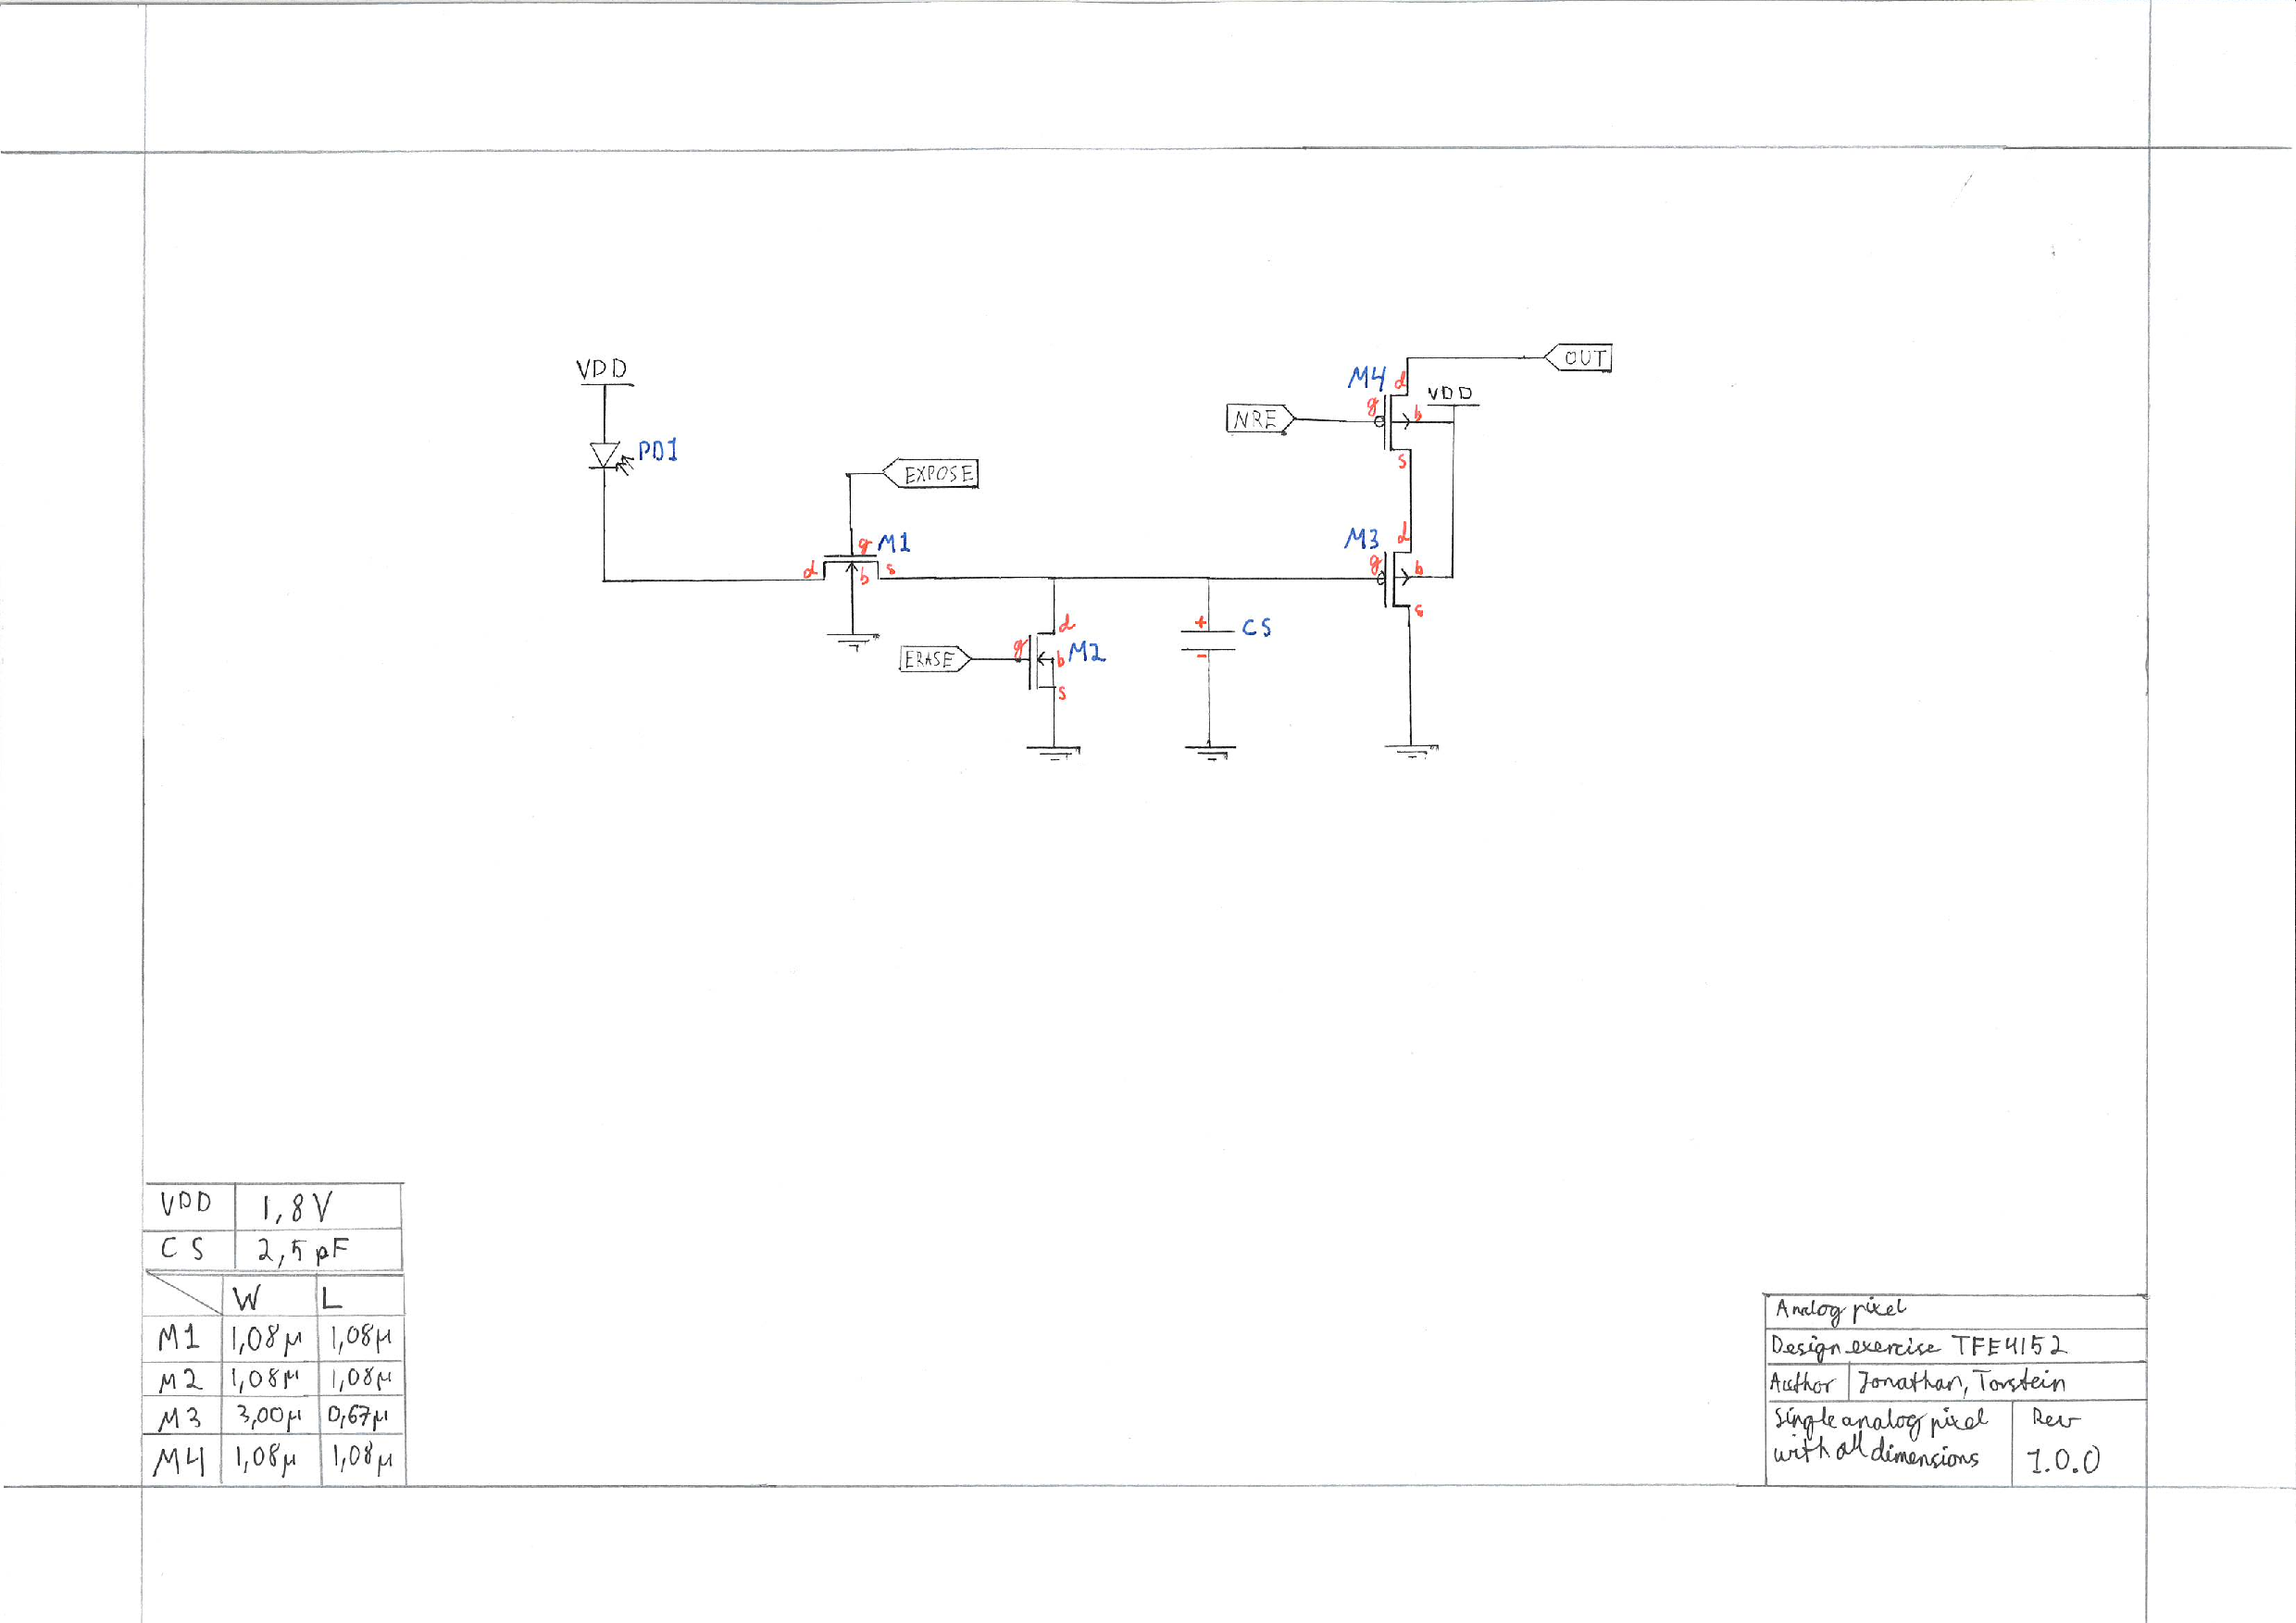
\includegraphics[width=0.95\textwidth]{figures/SchematicPixel}
  \caption{Implementation of one pixel, figure also exist in Appendix~\ref{ap:Schematics}}\label{fig:implpixel}
\end{figure}
\begin{figure}[htbp]
  \centering
  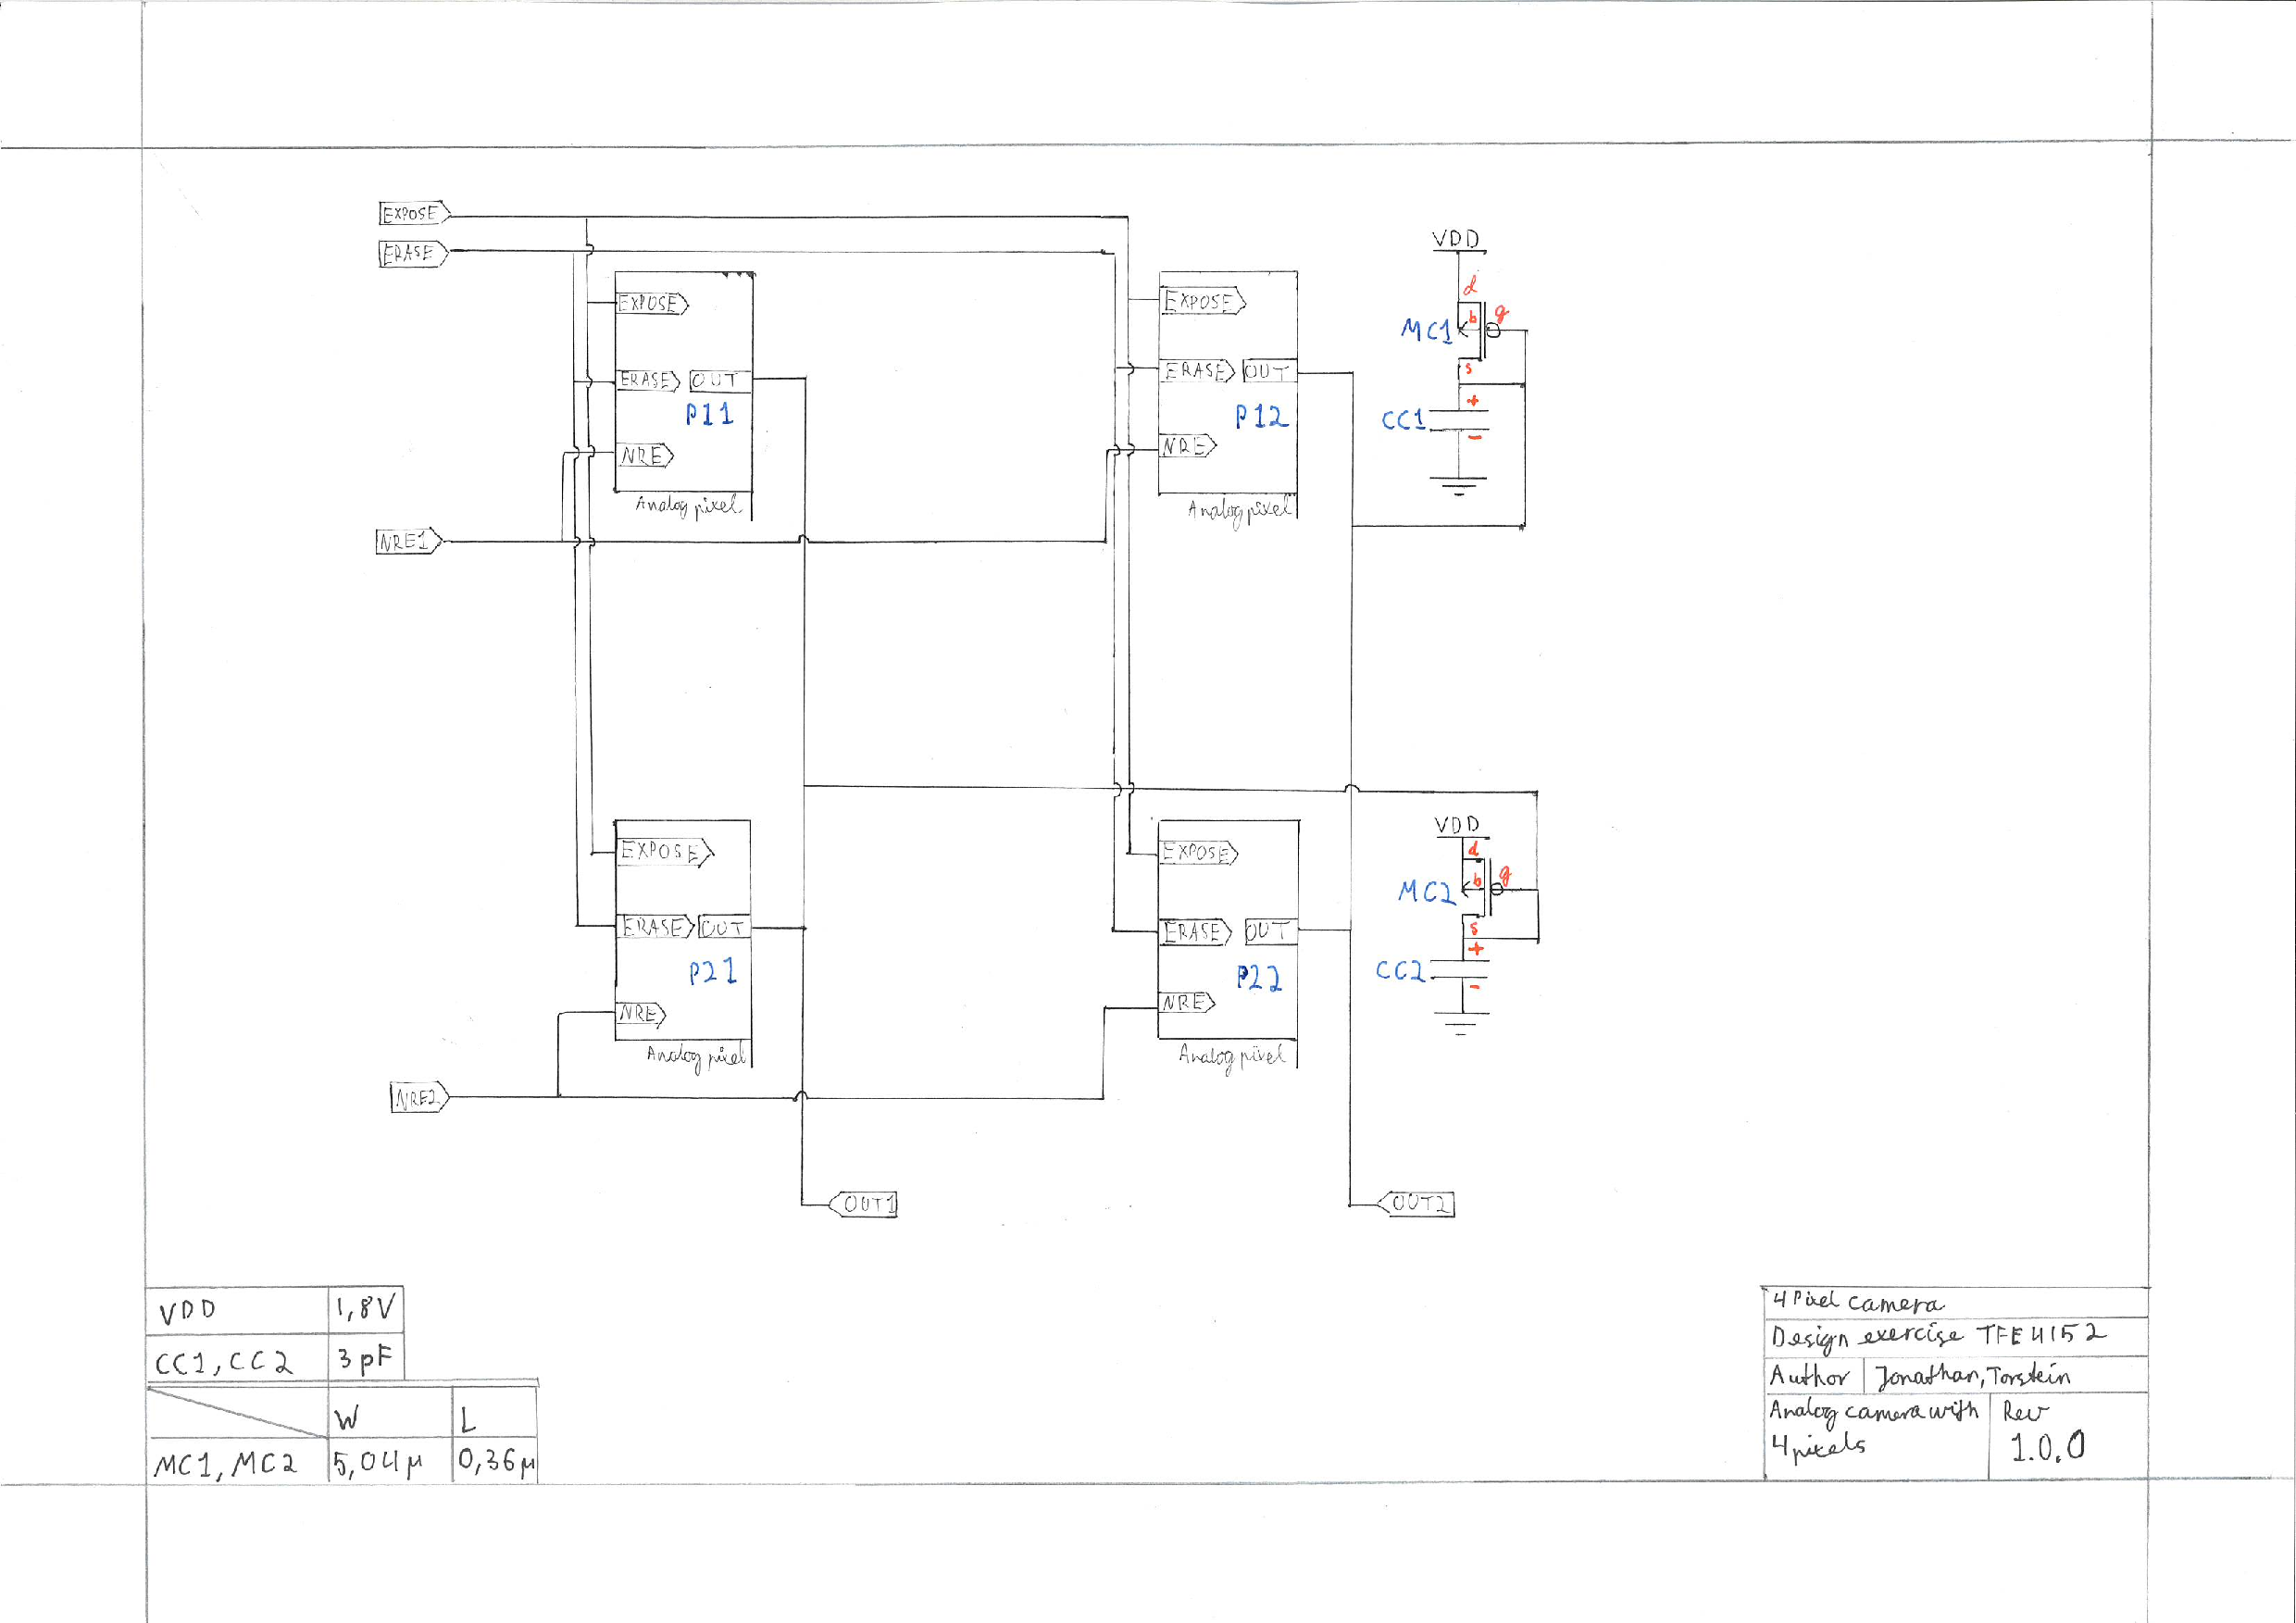
\includegraphics[width=0.85\textwidth]{figures/SchematicCamera}
  \caption{Implementation of the analog part of the camera, figure also exist in Appendix~\ref{ap:Schematics}}\label{fig:implcamera}
\end{figure}



\subsection{Transistor dimensions}

The most important property of the analog pixel is that the charge stored over CS remains unchanged while being read,
the transistors M1 and M2 must therefore be tuned for minimal leakage current as described in Section~\ref{sec:leakagecurrent}.
The transistors are limited by the technology used and must be in range: $0.3 \mskip3mu \mu m < L < 1.080 \mskip3mu \mu m$ and $1.080 \mskip3mu \mu m < W < 5.040 \mskip3mu \mu m $. This can be found in~\cite{oppgave}.
The transistor M4 must be tuned in the same way to avoid any interference between P11 and P21 as well as between P12 and P22 during readout as shown in figure~\ref{fig:implcamera}.
Though the analog design assumes a perfect production line, it should work for typical transistors seeing as the main principles of the design would still work.

The choice of physical dimensions are showed in table~\ref{tab:transcomponentvalues}.

\begin{table}[H]
  \centering
  \caption{Physical values of transistors}
  \begin{tabular}{ c | c c }
    Component & W[m] & L[m] \\
    \midrule
    M1 & $1.08\mu$ & $1.08\mu$ \\
    M2 & $1.08\mu$ & $1.08\mu$ \\
    M3 & $3.00\mu$ & $0.67\mu$ \\
    M4 & $1.08\mu$ & $1.08\mu$ \\
    MC1 & $5.04\mu$ & $0.36\mu$ \\
    MC2 & $5.04\mu$ & $0.36\mu$
  \end{tabular}
  \label{tab:transcomponentvalues}
\end{table}



\subsection{Values for capacitors}

The capacitors will be scaled to have maximum dynamic range. We know that the exposure time  will be between $2 \mskip3mu ms$ and $30 \mskip3mu ms$, and the capacitor should charge linearly until the exposure time is reached.
If the capacitance is too low, the capacitor will be fully charged before the full exposure time has passed which is not ideal.
This needs to be correct for at least one exposure time for all possible light levels described in~\cite{oppgave}.
The capacitance for CS was manually tuned for maximum bandwidth in simulation, see Section~\ref{sec:Simulations}.

The current source transistors MC1 and MC2 must be tuned for the quickest possible response of the current source, this is in order to get the fastest possible stable output when reading from a pixel.
They are therefore tuned for maximum current throughput as explained in Section~\ref{sec:leakagecurrent} and verified in Section~\ref{sec:Simulations}.

\begin{table}[htbp]
  \centering
  \caption{Capacitance of capacitors}
  \begin{tabular}{c | c}
    Component & C[F] \\
    \midrule
    CS & $2.5 \mskip3mu pF$ \\
    CC1 & $3.0 \mskip3mu pF$ \\
    CC2 & $3.0 \mskip3mu pF$
  \end{tabular}\label{tab:capcomponentvalues}
\end{table}
